\documentclass[11pt]{article}
\usepackage[utf8]{inputenc} % LaTeX source encoded as UTF-8
\usepackage[czech]{babel}

\usepackage{graphicx} %graphics files inclusion
\usepackage{amsmath} %advanced maths
\usepackage{amssymb} %additional math symbols
\usepackage{amsfonts}
\usepackage{listings}
\usepackage{hyperref}
\usepackage{color}
\usepackage{graphicx}

\lstset{
	inputencoding=utf8,
	keywords={end,if,for,in,sort, return, and, then},
	keywordstyle=\color{black}\bfseries\em,
}

\begin{document}

\title{3. úloha -- Experimentální hodnocení kvality algoritmů}
\author{Ondřej Červenka}
\date{9. 12. 2015}
\maketitle

\section{Specifikace úlohy}

Mějme počet věcí $n \in \mathbb{N}$ a maximální váhu batohu $M \in \mathbb{N}$. \newline Každá věc $i \in \{1, 2, \ldots, n\}$ má určenou váhu $V_i \in \mathbb{N}$ a cenu $C_i \in \mathbb{N}^0$. Úkolem je najít takovou kombinaci věcí, která má co nejvyšší hodnotu a zároveň nepřekračuje maximální váhu batohu $M$.

Problém budeme řešit ve variantě $0/1$, tedy každou věc máme k dispozici pouze jednou. Řešením jsou tedy čísla $\{x_1, x_2, \ldots, x_n\}$, $x_i \in \{0,1\}$ pro která platí $$\sum_{i=1}^n x_iV_i \leq M$$ a zároveň $$\sum_{i=1}^n x_iC_i = max $$ kde $max$ je maximální možná cena.

\section{Měřené algoritmy}
\label{sec:alg}

Při měření časové náročnosti se zaměříme především na algoritmus využívající metodu větví a hranic (branch \& bound)\footnote{Moje implementace tohoto algoritmu kromě prořezávání stavového prostoru podle cenové funkce také nesestupuje ve větvích rekurze, kde je jisté, že přidání předmětu přetíží batoh. Je tedy o něco více datově závislá.} a algoritmus založený na dekompozici podle váhy. 

Mnou implemenotvané řešení hrubou silou není co se týče datových závislostí nijak zajímavé, neboť neprovádí žádné prořezávání stavového prostoru (ani podle omezení na maximální váhu batohu), a je tedy závislé pouze na počtu předmětů $n$ (vždy vyzkouší všech $2^n$ kombinací věcí a z nich vybere tu nejlepší, která splňuje omezení).

U greedy heuristiky nás bude zajímat především vliv vstupních dat na relativní chybu algoritmu. Na rozdíl od hrubé síly zde však existuje jistý vliv vstupu na dobu běhu, jelikož heuristika využívá datově závislý quicksort. Heuristiku nicméně budeme měřit zvlášť, jelikož doba jejího běhu je výrazně nižší než u ostatních algoritmů.

\subsection{Podmínky měření}

Algoritmy byly implementovány v C a kompilovány pomocí gcc 5.1.1. Při kompilaci nebyly použity žádné optimalizační přepínače. Program byl zkompilován a spouštěn na operačním systému GNU/Linux (Fedora) 64bit s verzí jádra 4.2.6. Procesor počítače je Intel Core i7-4510U s frekvencí 3.1 GHz.

Časy běhu byly získány pomocí funkce $clock()$ z knihovny $time.h$.

\section{Vliv vstupních dat na dobu běhu}

\subsection{Vliv maximální váhy}
\label{sec:maxw}
Vliv maximální váhy jsem testoval na 10 náhodných instancích vytvořených generátorem s paremetrem $W$ měnícím se v rozsahu od 100 do 2000. Ostatní paramtery byly nastaveny na pevné hodnoty ($m = 0.5$, $k = 1$, $d = 0$, $C = 100$). Počet věcí v batohu byl 30.

Z grafu \ref{fig:exact_times_weight} můžeme vidět, že vliv maximální váhy na algoritmus využívající dekompozici podle ceny je zcela minimální. To se dalo očekávat, neboť složitost algoritmu je $O(n^2 \cdot C_m)$, kde $C_m$ je maximální cena. Váhy předmětů nám tedy pouze určí hodnoty v tabulce, ale neovlivní její velikost a tak rychlost jejího procházení.

Vliv měnící se maximální váhy na běh branch \& bound algoritmu se zdá výraznější, nevyplívá z něj však žádná závislost času běhu na rostoucí maximální váze. Větší výkyvy oproti dynamickému algoritmu se dají vysvětlit náhodně generovanými cenami a váhami, které ovlivňují dobu běhu. 

U dynamického algoritmu tyto nehrají žádnou roli a záleží jen na maximální ceně\footnote{Ve skutečnosti nám velikost tabulky a tím i délku výpočtu spíše než maximální cena určuje suma všech cen předmětů v instanci (a tedy $C_m \cdot n$ představuje pouze horní mez). Jestliže generátor generuje ceny předmětů rovnoměrně, na tomto rozdílu tolik nezáleží, zajímal by nás až kdybychom generovali instance s nerovnoměrně rozloženými cenami (více předmětů s cenou výrazně nižší než je maximum by nás vzdálilo od horní meze).} a počtu předmětů. Proto je chování dynamického algoritmu stabilnější.

Z grafu \ref{fig:exact_times_weight} by se také mohlo zdát, že je dynamický algoritmus je rychlejší. To je však dáno tím, že parametr $C$ (maximální cena) náhodného generátoru je nastaven na relativne nízkou pevnou hodnotu (100). 
Zvětšením této hodnoty bychom mohli graf libovolně posunout po ose $y$.

Vliv maximální váhy na dobu výpočtu greedy heuristiky je podobný jako u breach \& bound algoritmu, jak můžeme vidět na grafu \ref{fig:greedy_weight}. Ani zde nelze pozorovat žádnou závislost.

\begin{figure}[h!]
	\centering
    	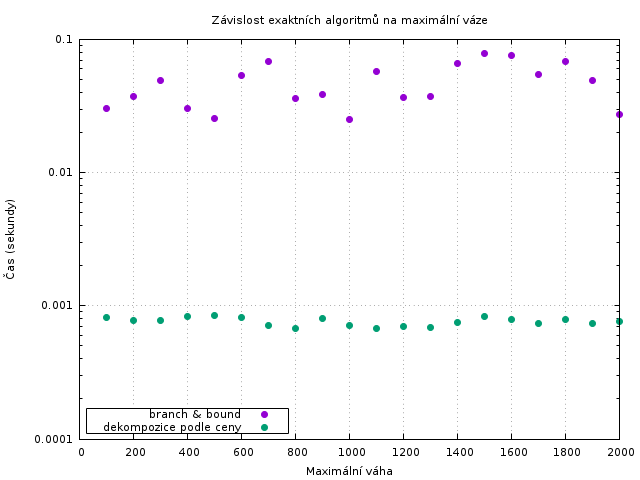
\includegraphics[width=0.8\textwidth]{../data/max_weight_times.png}
	\caption{Vliv maximální váhy na čas pro exaktní algoritmy, rozsah 100 - 2000}
	\label{fig:exact_times_weight}
\end{figure}

\begin{figure}[h!]
	\centering
    	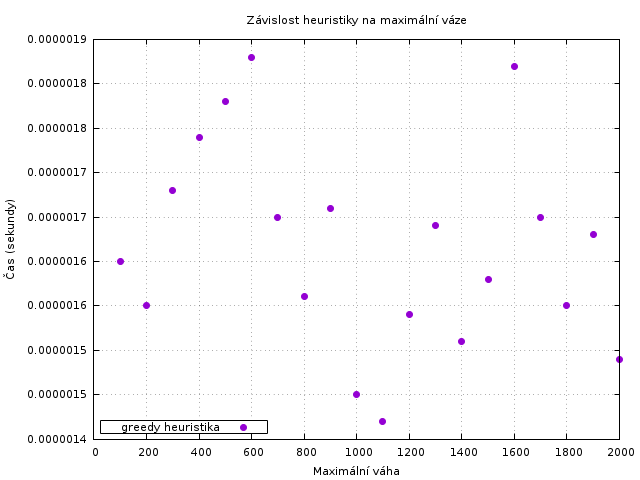
\includegraphics[width=0.8\textwidth]{../data/greedy_weight.png}
	\caption{Vliv maximální váhy na čas pro greedy heuristiku, rozsah 100 - 2000}
	\label{fig:greedy_weight}
\end{figure}

\subsection{Vliv maximální ceny}
\label{sec:maxp}

Při měření vlivu maximální ceny byly parametry náhodného generátoru instancí nastaveny stejně jako je popsáno v sekci \ref{sec:maxw}, s tím rozdílem, že parametr $W$ byl zafixován na hodnotu 100 a parametr $C$ byl škálován od 100 do 2000. 

Podle grafu \ref{fig:exact_times_price} je vliv maximální ceny na dobu běhu branch \& bound algoritmu podobný jako vliv maximální váhy.

Vliv na dynamický algoritmus jasně vyplívá z jeho složitosti $O(n^2 \cdot C_m)$, a je tedy lineární. I zde platí, že graf můžeme posunout, tentokrát změnou nastavení rozsahu maximálních vah. Takovou změnu a její vliv na dobu běhu lze vidět na grafu \ref{fig:price20000}, kde se maximální cena mění v rozsahu od 1000 do 20000.

Je vidět, že pro vyšší maximální cena začíná být výhodnější branch \& bound algoritmus.

Ani zde se neprokázala žádná závislost doby běhu greedy algoritmu na zvolené maximální ceně, což ukazuje graf \ref{fig:greedy_price}.

\begin{figure}[h!]
	\centering
    	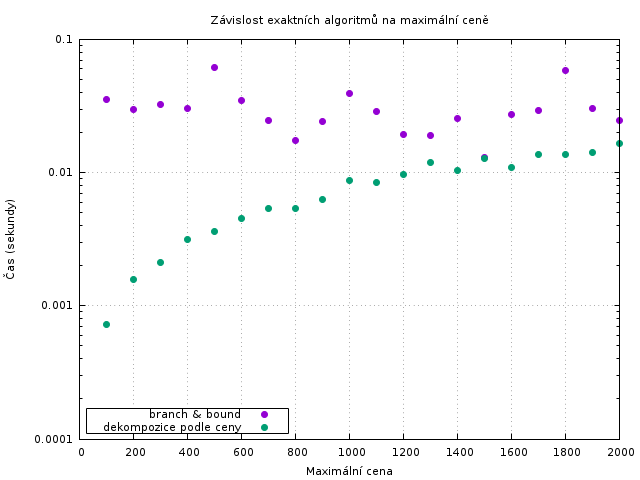
\includegraphics[width=0.8\textwidth]{../data/max_price_times.png}
	\caption{Vliv maximální ceny na čas pro exaktní algoritmy, rozsah 100 -- 2000}
	\label{fig:exact_times_price}
\end{figure}

\begin{figure}[h!]
	\centering
    	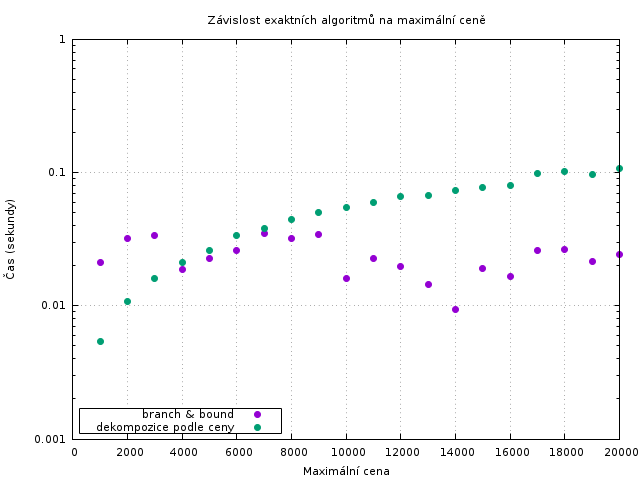
\includegraphics[width=0.8\textwidth]{../data/max_price_times20000.png}
	\caption{Vliv maximální ceny na čas pro exaktní algoritmy, rozsah 1000 -- 20000}
	\label{fig:price20000}
\end{figure}

\begin{figure}[h!]
	\centering
    	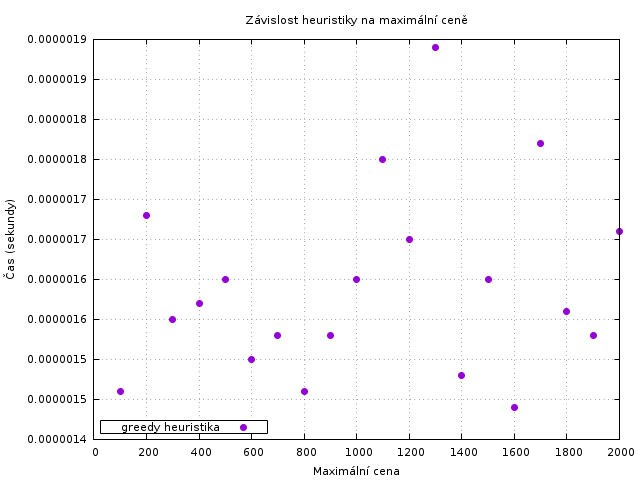
\includegraphics[width=0.8\textwidth]{../data/greedy_price.png}
	\caption{Vliv maximální ceny na čas pro greedy heuristiku, rozsah 1000 -- 20000}
	\label{fig:greedy_price}
\end{figure}

\subsection{Vliv poměru kapacity batohu a sumární váhy}

I v tomto testu byly parametry generátoru zafixovány na stejné hodnoty jako v sekcích \ref{sec:maxw} a \ref{sec:maxp} ($C$ i $W$ byly v tomto případě nastaveny na hodnotu 100). Parametr $m$ byl škálován v rozsahu od 0.05 do 0.95.

Podle očekávání poměr kapacity batohu a sumární váhy nemá žádný pozorovatelný vliv na dobu běhu dynamického algoritmu, jak je patrné z grafu \ref{fig:ratio1}. 

To je dáno opět dáno tím, že algoritmus vyplňuje celou tabulku velikosti $n^2 \cdot C_m$, bez ohledu na omezující podmínku. Ta je kontrolována až po vyplnění tabulky při výběru optimálního řešení.

Na grafu \ref{fig:ratio1} také můžeme pozorovat, že závislost branch \& bound algoritmu připomíná Gaussovu křivku. To je dáno způsobem implementace zmíněným v sekci \ref{sec:alg}. Stavový prostor je tedy prořezáván jak podle ceny, tak podle kapacity batohu.

Pokud je poměr kapacity k sumární váze malý, do batohu se vejde pouze malé množství a stavový prostor je ořezán podle omezující podmínky, která vyřadí stavy s větším množství věcí. Naopak pokud je poměr velký, do batohu se vejde většína věcí, a při prořezávání podle cenové funkce jsou odstraněny stavy s malým počtem věcí a tudíž i menší cenou.

Jak to dopadne, pokud bychom neprořezávali stavový prostor podle kapacity batohu můžeme vidět na grafu \ref{fig:ratiobb}\footnote{Kvůli rychlosti bylo měřeno na instancích s 25 věcmi}. Je vidět, že v při vyšších poměrech oba algoritmy fungují stejně, neboť většina stavového prostoru je ořezaná podle cenové funkce.

Naopak pro malé poměry je algoritmus bez prořezávání podle kapacity pomalejší, neboť neprořeže stavý, které přetěžují batoh. Těch je zde ale většina.

Na grafu \ref{fig:ratio_greedy} nelze pozorovat žádnou závislost doby běhu greedy algoritmu na poměru kapacity batohu a sumární váhy.

\begin{figure}[h!]
	\centering
    	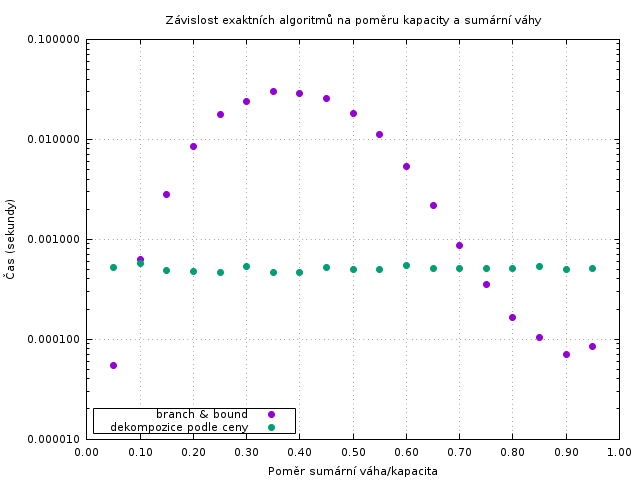
\includegraphics[width=0.8\textwidth]{../data/ratio1.png}
	\caption{Vliv poměru kapacity a sumární váhy na čas pro exaktní algoritmy}
	\label{fig:ratio1}
\end{figure}

\begin{figure}[h!]
	\centering
    	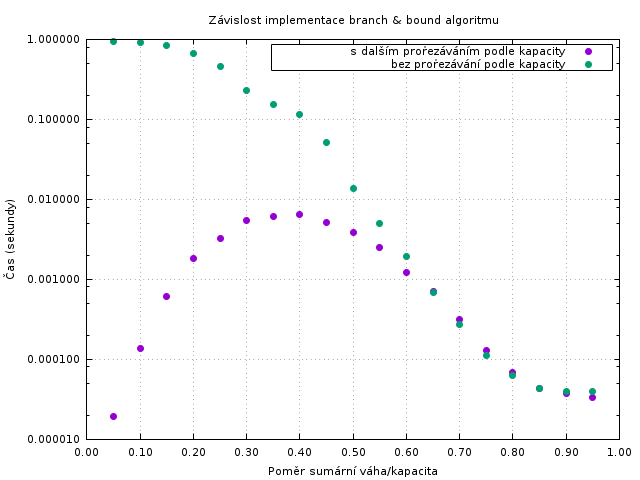
\includegraphics[width=0.8\textwidth]{../data/ratiobb.png}
	\caption{Porovnání vlivu poměru kapacity a sumární váhy na různe implementace branch \& bound algoritmu}
	\label{fig:ratiobb}
\end{figure}

\begin{figure}[h!]
	\centering
    	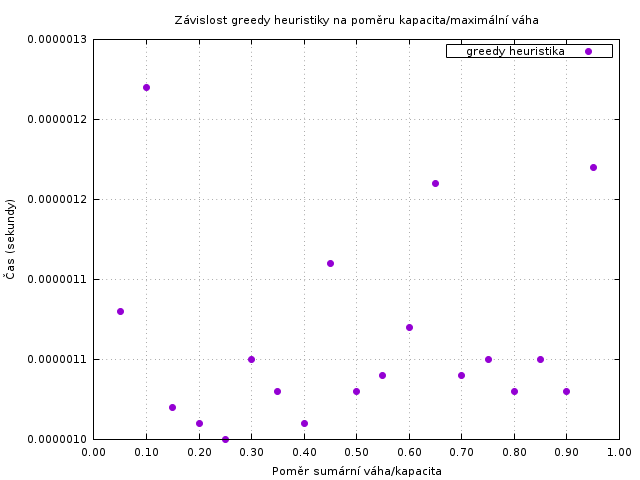
\includegraphics[width=0.8\textwidth]{../data/ratio_greedy.png}
	\caption{Vliv poměru kapacity a sumární váhy na čas pro greedy heuristiku}
	\label{fig:ratio_greedy}
\end{figure}

\subsection{Vliv granularity}

Při zkoumání vlivu granularity byly zafixovány všechny parametry kromě $k$. Ten nám udává jak velký význam hraje váha předmětu, když se rozhodujeme, zda předmět přidáme do instance.

Konkrétní vzorce jsou $p = \frac{1}{W^k}$ pokud generujeme instanci s převahou malých předmětů ($d = -1$) a 
$p = \frac{1}{W_m - W}$ pokud generujeme instanci s převahou velkých předmětů ($d = 1$), $p$ je pravděpodobnost, že předmět bude součástí instance, $W$ je váha předmětu, $W_m$ je maximální váha předmětu.

Pro $k = 1$ a $d = -1$ se tedy pravděpodobnost, že předmět bude součástí vygenerované instance snižuje lineárně s jeho váhou, pro $k = 2$ se snižuje kvadraticky. Pro $d = 1$ toto funguje analogicky.  

Graf \ref{fig:gran1} ukazuje, že rostoucí exponent dobu běhu obou testovaných algoritmů nikjak významně neovlivní. Zajímavý je však posun v časech u branch \& bound algoritmu. Ty jsou horší (instance s převahou velkých věcí) i lepší (instance s převahou malých věcí) než kdyby byly váhy vygenerovány rovnoměrně.

\begin{figure}[h!]
	\centering
    	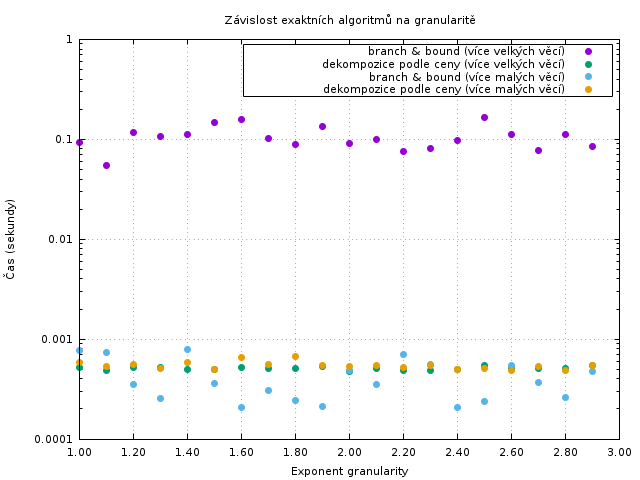
\includegraphics[width=0.8\textwidth]{../data/gran1.png}
	\caption{Vliv exponentu granularity na čas pro exaktní algoritmy, více velkých věcí}
	\label{fig:gran1}
\end{figure}

\section{Vliv vstupních dat na chybu heuristiky}

Výpočet relativní chyby $\epsilon$ byl proveden podle vzorce $\epsilon = \frac{C(OPT) - C(APX)}{C(OPT)}$, kde 
$C(OPT)$ je cena optimálního řešení a $C(APX)$ je cena řešení nalezeného greedy heuristikou.

Parametry generátoru instancí byly pro toto měření nastaveny tak, jak je popsáno v sekcích \ref{sec:maxw} a \ref{sec:maxp}

\subsection{Vliv váhy a ceny}

Jak je vidět na grafech \ref{fig:werror} a \ref{fig:perror}, nelze vyvodit žádnou souvislost mezi maximální cenou nebo maximální váhou a relativní chybou heuristiky. 

\begin{figure}[h!]
	\centering
    	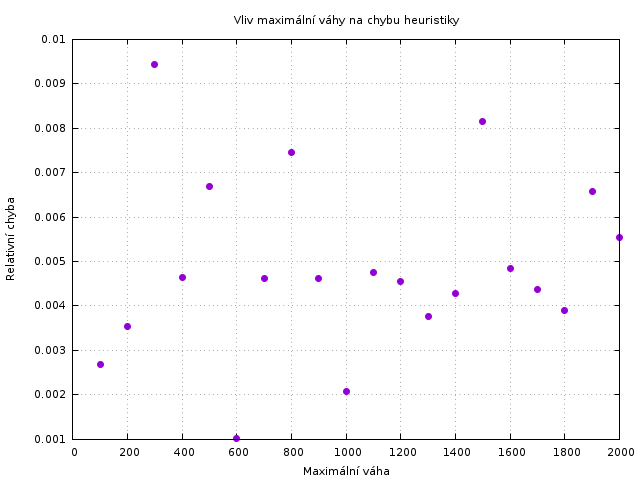
\includegraphics[width=0.8\textwidth]{../data/werror.png}
	\caption{Vliv maximální váhy na relativní chybu greedy heuristiky}
	\label{fig:werror}
\end{figure}


\begin{figure}[h!]
	\centering
    	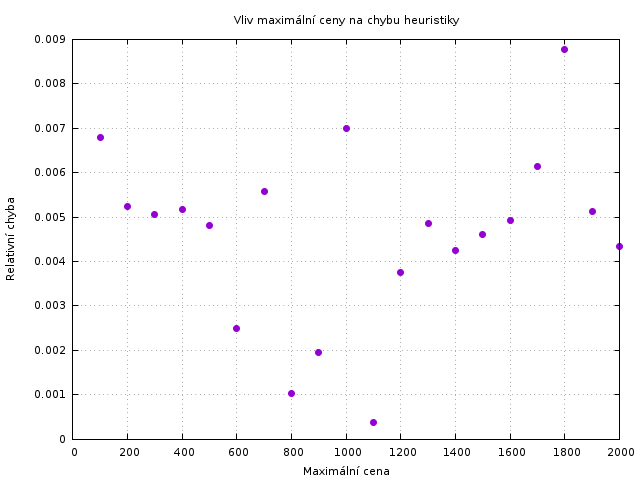
\includegraphics[width=0.8\textwidth]{../data/perror.png}
	\caption{Vliv maximální ceny na relativní chybu greedy heuristiky}
	\label{fig:perror}
\end{figure}

\subsection{Vliv poměru kapacity a sumární váhy batohu}
\label{sec:merror_sec}


Při testování vlivu poměru kapacity a sumární váhy na chybu heruristiky jsem se rozhodl vyzkoušet, jak se bude tento vliv lišit v případech s odlišnou granularitou. Předpokádal jsem, že instance s převahou malých věcí umožní batoh zaplnit efektivněji, což by mělo poskytnout výhodu greedy algoritmu (velké předměty s dobrým poměrem ceny a váhy nemusí batoh zaplnit efektivně).

Na grafu \ref{fig:merror} tedy kromě vlivu poměru na relativní chybu při rovnoměrně rozdělených věcech můžeme vidět i vliv při převaze malých a velkých věcí (exponent granularity $k$ byl nastaven na 2). Můžeme pozorovat, že většinou platí, že instance s převahou malých věcí vykazují menší relativní chybu, a to především pro malé poměry. 

S rostoucím poměrem chyba klesá, což se dá vysvětlit vyšším počtem věcí v batohu a tedy menším prostorem pro špatné rozhodnutí. Klesá také rozdíl v kvalitě řešní instancí s převahou maých nebo velkých věcí.

\begin{figure}[h!]
	\centering
    	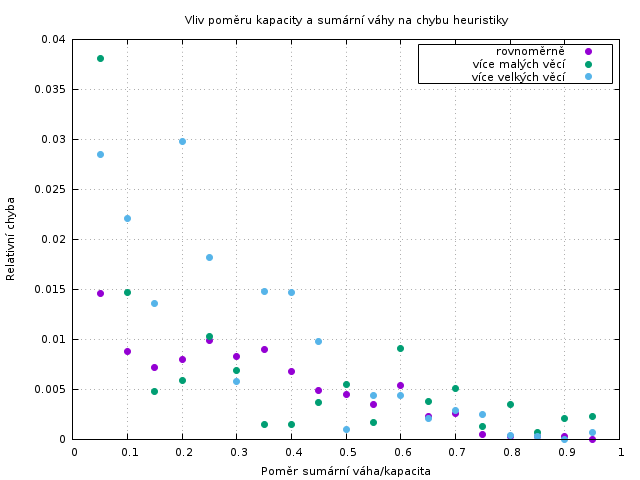
\includegraphics[width=0.8\textwidth]{../data/merror.png}
	\caption{Vliv poměru kapacity a sumární váhy na relativní chybu greedy heuristiky}
	\label{fig:merror}
\end{figure}

\subsection{Vliv granularity}

Na rozdíl od sekce \ref{sec:merror_sec} bylo toto měření provedeno na instancích s pevným parametren $m = 0.5$.
Z grafu \ref{fig:gerror} je vidět, že chyba greedy heuristiky při tomto poměru na granularitě věcí nezávisí, a to jak při převaze velkých tak při převaze malých věcí.

Zdá se tedy, že pro důkladnější ověření vliv granularity na kvalitu výsledku je třeba tento vliv kombinovat s vlivy dalších parametrů.

\begin{figure}[h!]
	\centering
    	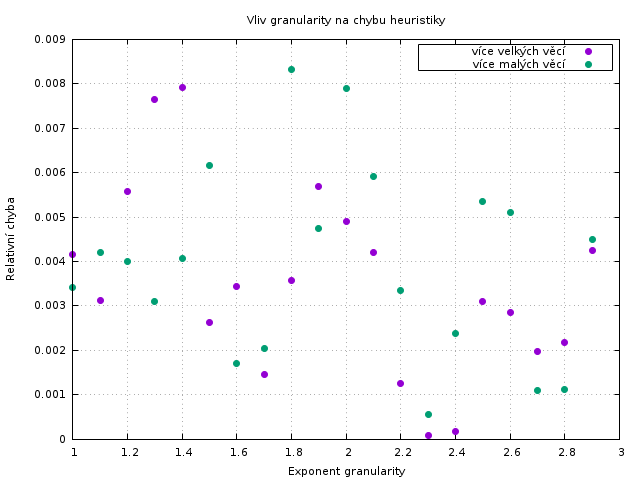
\includegraphics[width=0.8\textwidth]{../data/gerror.png}
	\caption{Vliv granulartiy na relativní chybu greedy heuristiky}
	\label{fig:gerror}
\end{figure}

\section{Závěr}

Ukázalo se tedy, že nejmenší vliv na chování testovaných algoritmů má maximální váha batohu. To je samozřejmě také dáno tím, že dynamický algoritmus využívá dekompozici podle ceny, nicméně ani ostatní algoritmy žádnou výraznou závislost na maximální váze nevykazovaly.

Maximální cena měla podle očekávání významný vliv na dobu běhu dynamického algoritmu, u ostatních algoritmů byly výsledky podobné jako u maximální váhy, vliv byl tedy neznatelný.

Dynamický algoritmus se také ukázal jako velice předvídatelný, neboť na dobu jeho běhu měla vliv skutečně jen maximální cena a počet předmětů. Algoritmus využívající metodu branch \& bound byl více ovlivněn náhodně generovaným vstupem (i bez ohledu na parametry generátoru).

Doba běhu branch \& bound algoritmu byla nejvíce závsilá na poměru kapacity batohu a sumární váhy všech předmětů, jelikož tento parametr nejvíce ovlivnil míru prořezání stavového prostoru.

Granularita také nijak významě neovlivnila dobu běhu algoritmů, zajímavý výsledek poskytla pouze volba převahy menších či větší předmětů. Zde se ukázalo, že branch \& bound algoritmus dosahuje lepších výsledků při převaze malých věcí.

Doba běhu greedy heuristky byla také nezávislá na nastavení parametrů generátoru instancí. To bylo možné očekávat, neboť hlavní část výpočtu zde představuje quicksort. Doba jeho běhu je sice závislá na vstupních datech, ne však takovým způsobem, aby se dala ovlivnit nastavením generátoru.

Výsledky zkoumání relativní chyby heuristiky byly méně přesvědčivé. Ukázalo se, že chyba je ovlivněna především poměrem kapacity a sumární váhy, další významné závislosti se však najít nepodařilo.

\end{document}
